\chapter{泊松括号、生成元与角动量}

\lectureoverview{泊松括号不仅仅是一种紧凑地改写哈密顿方程的方式。它是一种生成变换的代数运算。与哈密顿量作括号运算生成时间演化；与动量作括号运算生成平移；与角动量作括号运算生成旋转。在这种语言中，对称性与守恒成为同一个消失的括号的两种解读。我们将从谐振子出发发展这一思想，然后利用角动量代数在不引入欧拉角的情况下得到陀螺进动。}

\section{沿哈密顿轨迹的函数}

设
\[
  F=F(q_1,\ldots,q_n,p_1,\ldots,p_n)
\]
是相空间上充分可微的函数。可以从两个角度来看待它。第一，它为相空间的每一点赋予一个数。第二，一旦选定了一条哈密顿轨迹，由于点\((q(t),p(t))\)在运动，它就变成了时间的函数。沿该轨迹，
\begin{equation}
  \frac{dF}{dt}
  =
  \sum_i\left(
    \frac{\partial F}{\partial q_i}\dot q_i
    +\frac{\partial F}{\partial p_i}\dot p_i
  \right).
  \label{eq:l8-chain-rule}
\end{equation}
哈密顿方程，
\begin{equation}
  \dot q_i=\frac{\partial H}{\partial p_i},
  \qquad
  \dot p_i=-\frac{\partial H}{\partial q_i},
  \label{eq:l8-hamilton-equations}
\end{equation}
将其变为
\begin{equation}
  \frac{dF}{dt}
  =
  \sum_i\left(
    \frac{\partial F}{\partial q_i}
    \frac{\partial H}{\partial p_i}
    -
    \frac{\partial F}{\partial p_i}
    \frac{\partial H}{\partial q_i}
  \right).
  \label{eq:l8-fdot-expanded}
\end{equation}
右端的组合在整个经典力学中都会出现，即使其中任何一个位置都不是哈密顿量。这促使我们定义
\begin{equation}
  \boxed{
  \{F,G\}
  =
  \sum_i\left(
    \frac{\partial F}{\partial q_i}
    \frac{\partial G}{\partial p_i}
    -
    \frac{\partial F}{\partial p_i}
    \frac{\partial G}{\partial q_i}
  \right).}
  \label{eq:l8-poisson-definition}
\end{equation}
因此式~\eqref{eq:l8-fdot-expanded}为
\begin{equation}
  \boxed{\dot F=\{F,H\}.}
  \label{eq:l8-time-generator}
\end{equation}

\begin{classroomqa}
  \audiencequestion{如果将第二个位置从\(H\)改为任意函数\(G\)，该括号是否仍是\(F\)的时间导数？
  \lecturetimestamp{00:05:45--00:06:15}}
  \lecturerresponse{不是。在记号被推广的过程中，听众抓住了一个要点。式~\eqref{eq:l8-poisson-definition}
  对任意两个相空间函数定义了\(\{F,G\}\)，但
  \(\dot F=\{F,G\}\)仅在\(G\)是哈密顿量时成立。一般的
  \(G\)将生成不同的无穷小变换。}
\end{classroomqa}

将时间的微小变化写成
\begin{equation}
  \delta_t F=\epsilon\,\{F,H\}.
  \label{eq:l8-small-time-step}
\end{equation}
是有用的。这一形式预示了后面的内容。时间演化是由泊松括号生成的更大变换族中的一个成员。

\section{括号的代数}

现在可以把括号当作一种自身的演算来使用。它的规则来自普通微分：
\begin{align}
  \{A,B\}&=-\{B,A\}, \label{eq:l8-antisymmetry}\\
  \{A+B,C\}&=\{A,C\}+\{B,C\}, \label{eq:l8-additivity}\\
  \{\lambda A,B\}&=\lambda\{A,B\},
    \quad \lambda\ \text{constant}, \label{eq:l8-scalar-rule}\\
  \{AB,C\}&=A\{B,C\}+\{A,C\}B. \label{eq:l8-leibniz}
\end{align}
这四行分别表达了反对称性、可加性、乘以常数下的线性性以及莱布尼茨法则。经典相空间函数可交换地相乘，因此最后一行中普通因子\(A\)和\(B\)的位置无关紧要。在量子力学中对算符而言这不再成立。反对称性还意味着
\begin{equation}
  \{A,A\}=0.
  \label{eq:l8-self-bracket}
\end{equation}

对于正则坐标，基本括号为
\begin{equation}
  \boxed{
  \{q_i,q_j\}=0,\qquad
  \{p_i,p_j\}=0,\qquad
  \{q_i,p_j\}=\delta_{ij}.}
  \label{eq:l8-canonical-brackets}
\end{equation}
任何只依赖于\(q_i\)的函数与任何只依赖于\(q_i\)的函数的括号为零；对于只依赖于\(p_i\)的函数也有类似的说法。非零括号要求一个正则坐标与其共轭动量相遇。式~\eqref{eq:l8-canonical-brackets}中的克罗内克{\proseunicodefont δ}记录了只有指标匹配时才相遇。

\subsection{作为检验的谐振子}

考虑
\begin{equation}
  H=\frac{p^2}{2m}+\frac{kq^2}{2}.
  \label{eq:l8-oscillator-hamiltonian}
\end{equation}
现在我们刻意只使用括号规则和式~\eqref{eq:l8-time-generator}。首先，
\begin{align}
  \dot q
  &=\{q,H\}\\
  &=\frac{1}{2m}\{q,p^2\}\\
  &=\frac{1}{2m}\left(p\{q,p\}+\{q,p\}p\right)\\
  &=\frac{p}{m}.
  \label{eq:l8-qdot-oscillator}
\end{align}
势能项消失，因为\(\{q,q^2\}=0\)。类似地，
\begin{align}
  \dot p
  &=\{p,H\}\\
  &=\frac{k}{2}\{p,q^2\}\\
  &=\frac{k}{2}\left(q\{p,q\}+\{p,q\}q\right)\\
  &=-kq.
  \label{eq:l8-pdot-oscillator}
\end{align}
负号正是反对称性
\(\{p,q\}=-\{q,p\}=-1\)。将两个一阶方程合并得到
\begin{equation}
  m\ddot q=-kq.
  \label{eq:l8-hooke-equation}
\end{equation}

\begin{figure}[htbp]
  \centering
  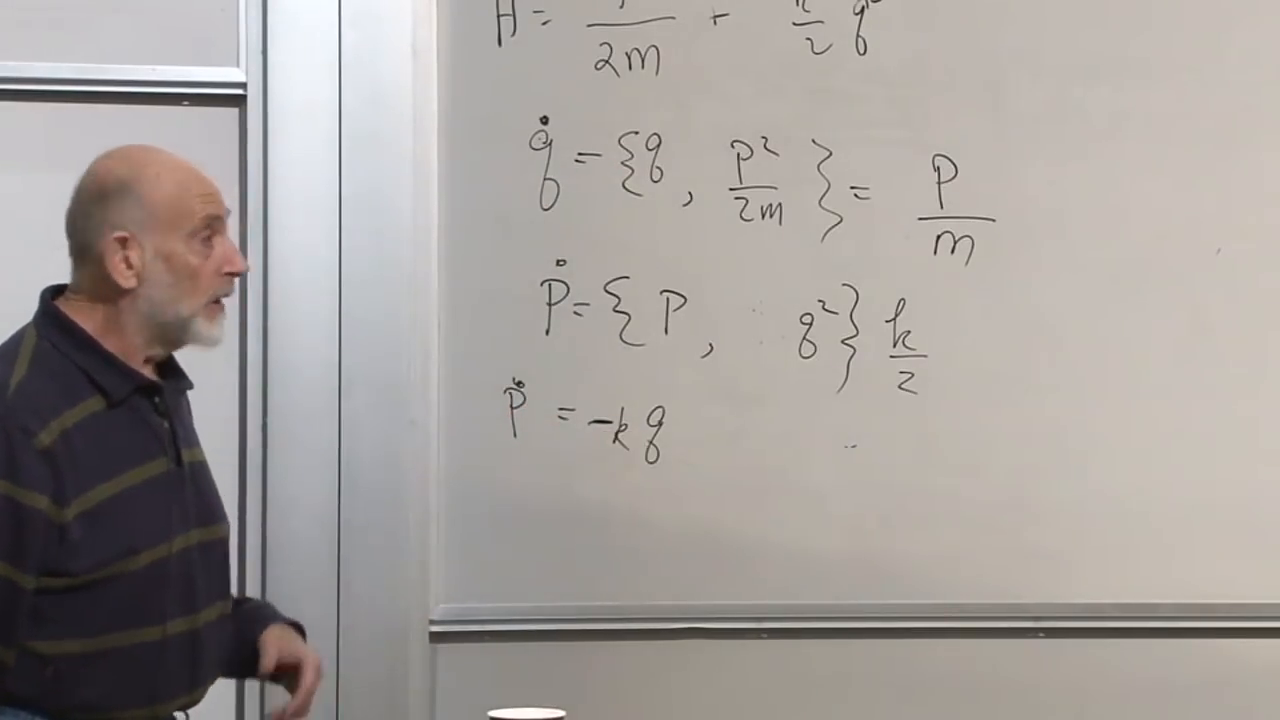
\includegraphics[width=0.82\textwidth]{lecture_08_figure_01.png}
  \caption{谐振子哈密顿量以及给出\(\dot q=p/m\)和\(\dot p=-kq\)的两次括号计算。}
  \lectureframe{00:23:20}
\end{figure}

在计算过程中，全班都在寻找一个意为\emph{取泊松括号}的动词，并暂时选定
\emph{泊松化}。这个玩笑标志着一次真正的观点转变：一旦知道了代数，就可以直接用它来运算，而不必从定义重新推导每一个结果。

\begin{classroomqa}
  \audiencequestion{这个数学结构是群，还是代数？它有逆元吗？\lecturetimestamp{00:23:48--00:24:16}}
  \lecturerresponse{它不是群：括号运算不提供所需的单位元和逆元。相空间函数构成一个泊松代数：它们具有普通的交换乘法和加法，以及一个满足莱布尼茨法则的反对称括号。另一个恒等式，即雅可比恒等式，补全了通常的抽象定义，尽管本讲并未展开。}
\end{classroomqa}

\begin{classroomqa}
  \audiencequestion{泊松括号与量子对易子之间有什么联系？\lecturetimestamp{00:24:18--00:25:00}}
  \lecturerresponse{本讲只给出一个预览。在向量子力学过渡时，经典括号被示意性地替换为
  \[
    \{A,B\}_{\mathrm{PB}}
    \longleftrightarrow
    \frac{1}{i\hbar}[\widehat A,\widehat B].
  \]
  这种对应关系需要关于算符排序和量子化的限定条件；这里并不是把它当作定理来使用。}
\end{classroomqa}

对于振子，该括号仅仅重新构造出了哈密顿方程。
它真正的经济性出现在生成元是除\(H\)之外的守恒量时。

\section{从旋转对称性重新得到角动量}

回忆本课程早先使用的诺特定理构造的无穷小形式。如果一个连续对称性使坐标变为
\begin{equation}
  \delta q_i=\epsilon F_i(q),
  \label{eq:l8-noether-variation}
\end{equation}
那么，在这里所考虑的设定中，其守恒量为
\begin{equation}
  G=\sum_i p_iF_i(q).
  \label{eq:l8-noether-charge}
\end{equation}
整体因子\(\epsilon\)可以省略：将一个守恒量乘以一个固定数不会改变守恒定律。

取一个粒子，使它绕\(z\)轴作无穷小旋转。按照本讲所用的取向，
\begin{equation}
  \delta x=-\epsilon y,\qquad
  \delta y=\epsilon x,\qquad
  \delta z=0.
  \label{eq:l8-z-rotation}
\end{equation}
式~\eqref{eq:l8-noether-charge}给出
\begin{equation}
  L_z=-p_xy+p_yx=xp_y-yp_x.
  \label{eq:l8-lz}
\end{equation}
轮换\(x\)、\(y\)和\(z\)，
\begin{equation}
  \boxed{\begin{aligned}
    L_x&=yp_z-zp_y,\\
    L_y&=zp_x-xp_z,\\
    L_z&=xp_y-yp_x.
  \end{aligned}}
  \label{eq:l8-angular-components}
\end{equation}
这些就是
\begin{equation}
  \boldsymbol L=\boldsymbol r\times\boldsymbol p.
  \label{eq:l8-cross-product}
\end{equation}的分量

\begin{figure}[htbp]
  \centering
  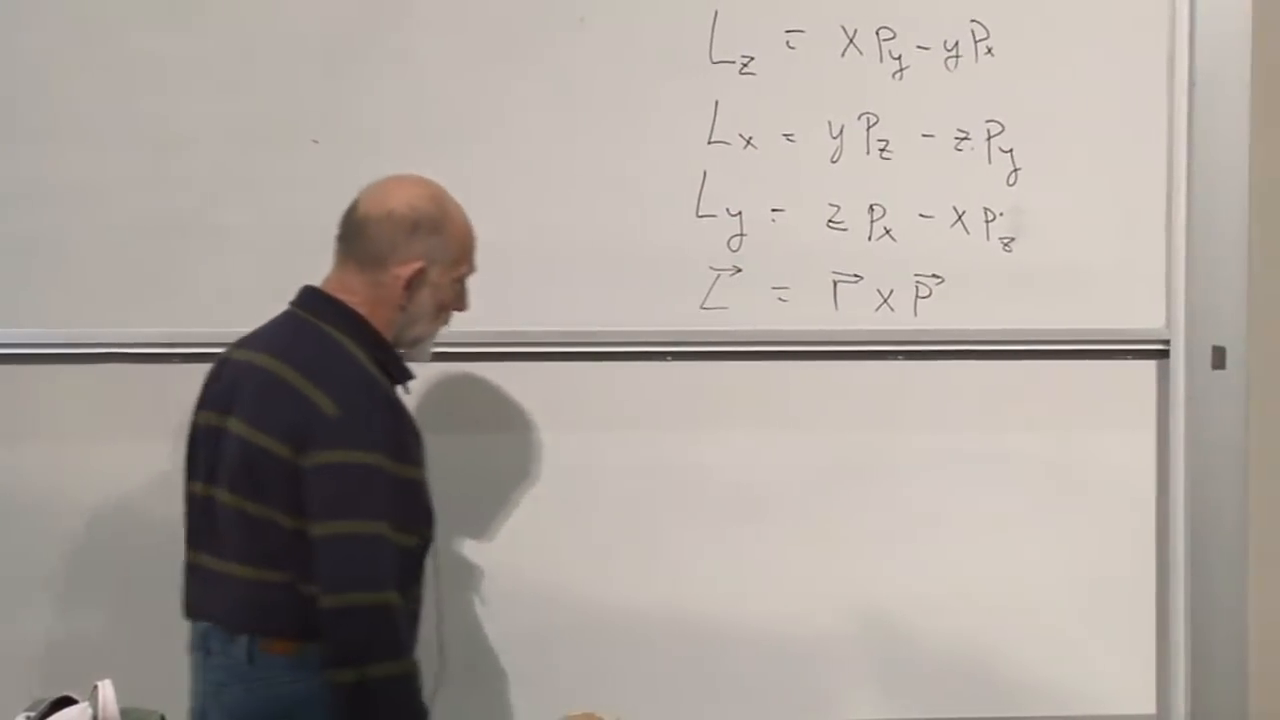
\includegraphics[width=0.82\textwidth]{lecture_08_figure_02.png}
  \caption{角动量的三个笛卡儿分量及其紧凑的叉积形式。}
  \lectureframe{00:34:00}
\end{figure}

绕任意单位向量\(\boldsymbol n\)的旋转由下式生成
\begin{equation}
  L_{\boldsymbol n}=\boldsymbol n\cdot\boldsymbol L.
  \label{eq:l8-arbitrary-axis}
\end{equation}
对于一个孤立的旋转不变系统，三个分量都守恒。如果只有绕某一个轴的旋转仍是对称性，那么只有沿该轴的分量被保证守恒。

\section{角动量生成旋转}

与其立即去解一个旋转动力学问题，不如让我们考察\(L_z\)在括号下起什么作用。利用式~\eqref{eq:l8-lz}，
\begin{align}
  \{x,L_z\}
  &=\{x,xp_y-yp_x\}
   =-y\{x,p_x\}
   =-y,\\
  \{y,L_z\}
  &=\{y,xp_y-yp_x\}
   =x\{y,p_y\}
   =x,\\
  \{z,L_z\}&=0.
  \label{eq:l8-position-rotation-brackets}
\end{align}
这些正是式~\eqref{eq:l8-z-rotation}中的系数。

\begin{figure}[htbp]
  \centering
  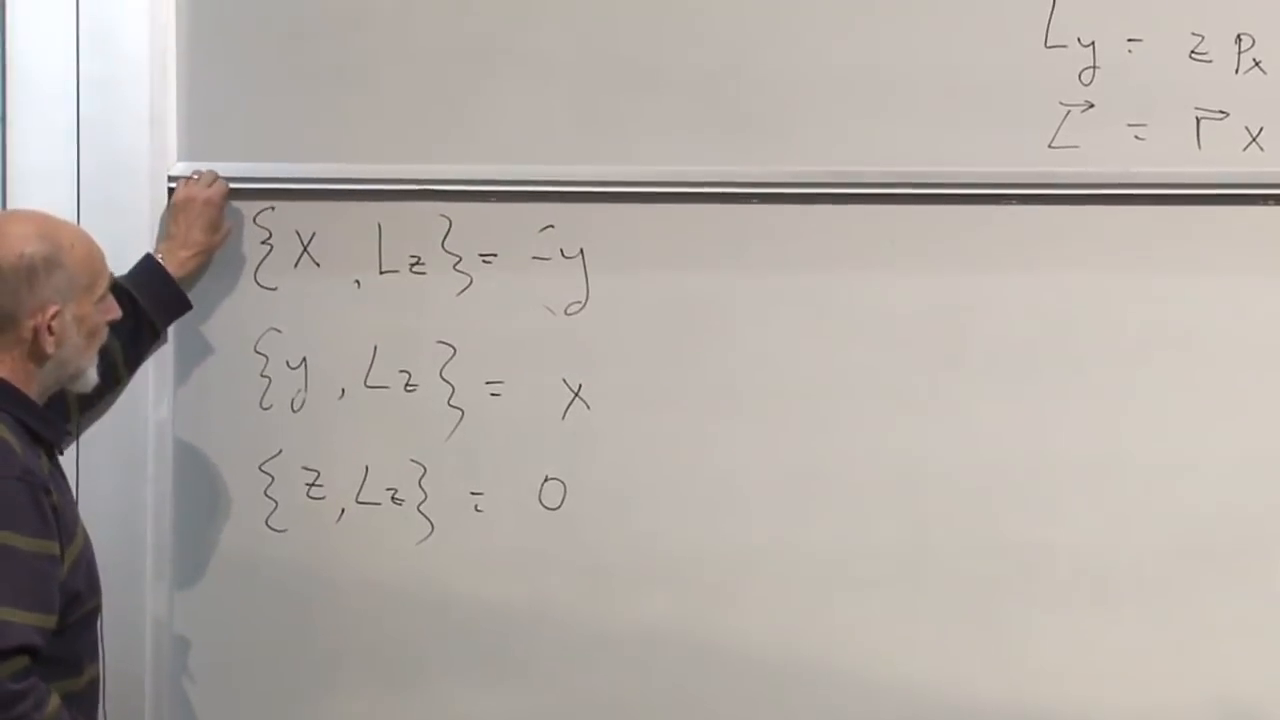
\includegraphics[width=0.82\textwidth]{lecture_08_figure_03.png}
  \caption{坐标与\(L_z\)的括号：该括号再现了\((x,y,z)\)的无穷小旋转。}
  \lectureframe{00:38:41}
\end{figure}

动量也是一个向量，同样的计算给出
\begin{equation}
  \begin{aligned}
    \{p_x,L_z\}&=-p_y,\\
    \{p_y,L_z\}&=p_x,\\
    \{p_z,L_z\}&=0.
  \end{aligned}
  \label{eq:l8-momentum-rotation-brackets}
\end{equation}

\begin{figure}[htbp]
  \centering
  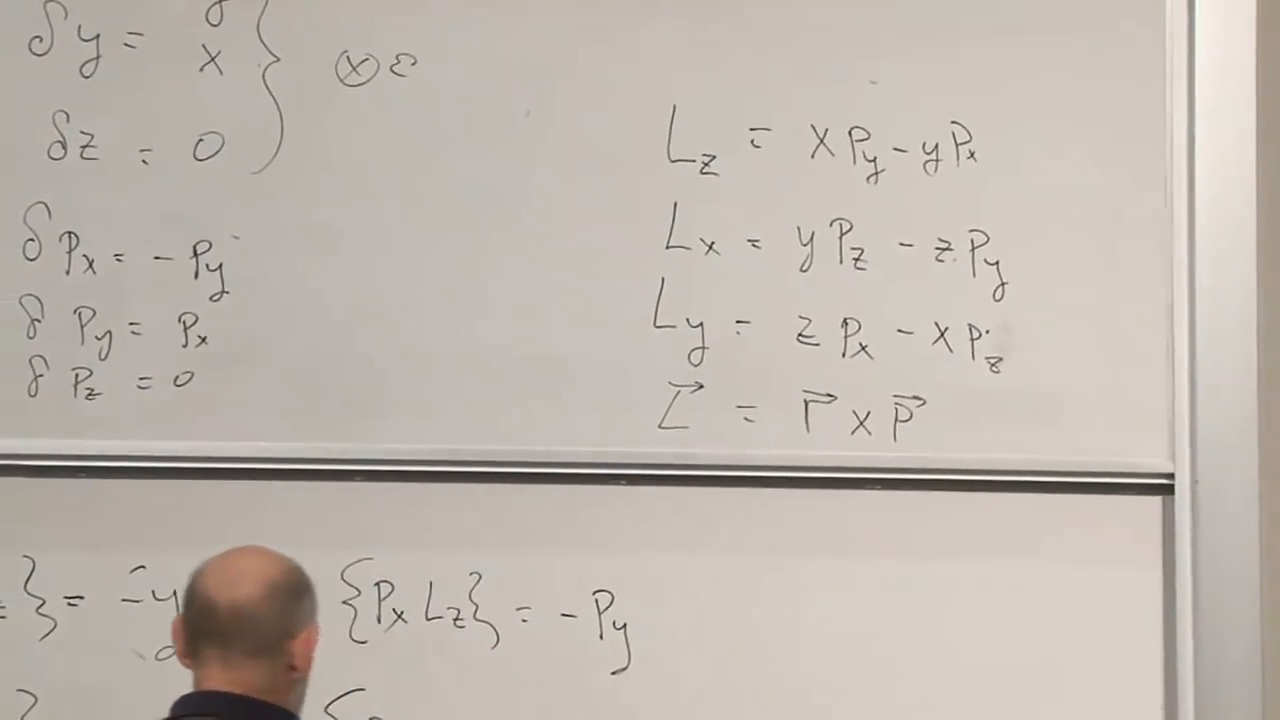
\includegraphics[width=0.82\textwidth]{lecture_08_figure_04.png}
  \caption{在由\(L_z\)生成的旋转下，位置和动量按相同的向量模式变换。}
  \lectureframe{00:42:08}
\end{figure}

因此，一般的哈密顿表述为
\begin{equation}
  \boxed{\delta_G A=\epsilon\{A,G\}.}
  \label{eq:l8-generator-rule}
\end{equation}
每一个相空间函数\(G\)都定义这样一个无穷小正则变换。如果\(G=L_z\)，它就是旋转。如果\(G=H\)，它就是时间中的一小步。

\begin{classroomqa}
  \audiencequestion{本讲有时说旋转系统，有时说旋转坐标。括号方程中采用的是哪一种约定？\lecturetimestamp{00:28:22--00:29:35}}
  \lecturerresponse{式~\eqref{eq:l8-z-rotation}确定了约定：它是无穷小主动旋转
  \((x,y)\mapsto(x-\epsilon y,y+\epsilon x)\)。坐标轴的被动旋转带有相反的符号。一旦约定确定，括号公式就没有歧义了。}
\end{classroomqa}

\section{动量生成平移}

在一个坐标中的平移有
\begin{equation}
  \delta q=\epsilon.
  \label{eq:l8-q-translation}
\end{equation}
这里式~\eqref{eq:l8-noether-variation}中\(F(q)=1\)，所以相应的守恒量为\(p\)。生成元的论断预言
\begin{equation}
  \{f(q),p\}=\frac{df}{dq}.
  \label{eq:l8-translation-derivative}
\end{equation}
本讲首先对幂用归纳法证明这一点。基例是\(\{q,p\}=1\)。假设
\begin{equation}
  \{q^{n-1},p\}=(n-1)q^{n-2}.
  \label{eq:l8-induction-hypothesis}
\end{equation}
那么乘积法则给出
\begin{align}
  \{q^n,p\}
  &=\{q\,q^{n-1},p\}\\
  &=q\{q^{n-1},p\}+\{q,p\}q^{n-1}\\
  &=(n-1)q^{n-1}+q^{n-1}\\
  &=nq^{n-1}.
  \label{eq:l8-power-translation}
\end{align}
线性性把结果推广到多项式和收敛的幂级数表示。更直接地，括号的定义对每一个可微的\(f(q)\)给出式~\eqref{eq:l8-translation-derivative}：
\begin{equation}
  \{f(q),p\}
  =
  \frac{\partial f}{\partial q}
  \frac{\partial p}{\partial p}
  =f'(q).
\end{equation}

\begin{figure}[htbp]
  \centering
  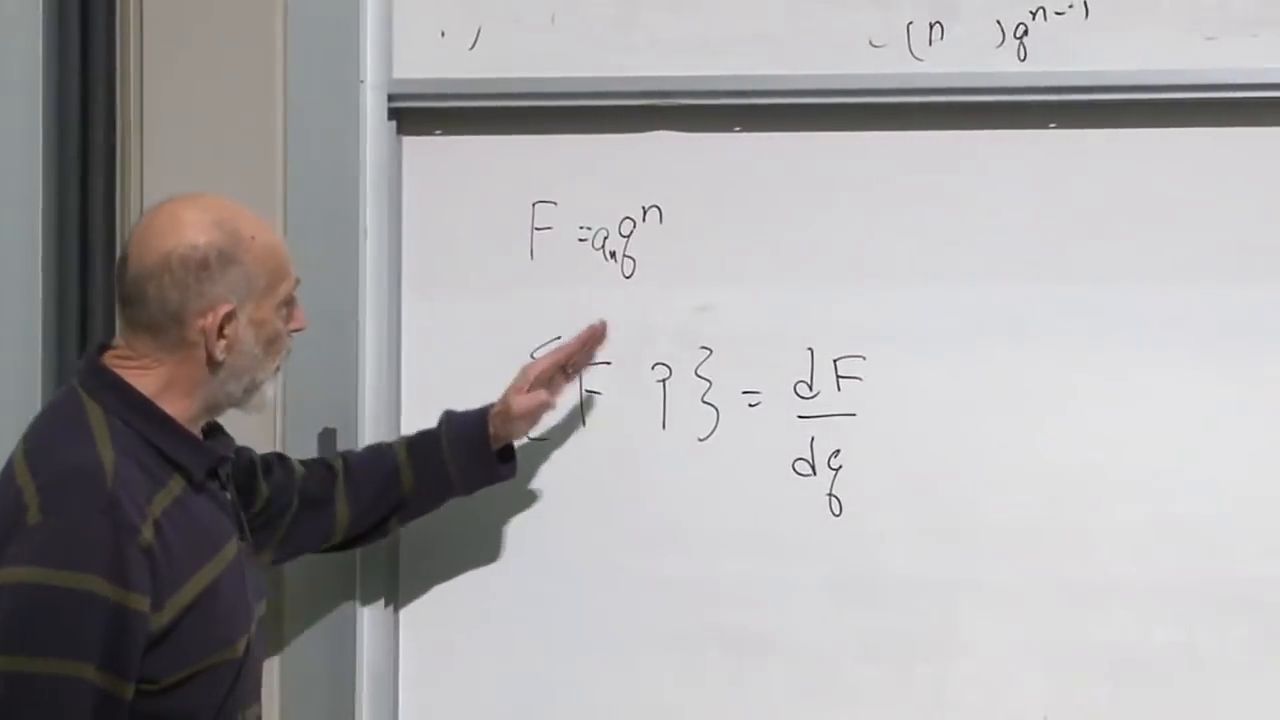
\includegraphics[width=0.82\textwidth]{lecture_08_figure_05.png}
  \caption{归纳论证之后的平移结果：
  \(\{F(q),p\}=dF/dq\)。}
  \lectureframe{00:53:18}
\end{figure}

我们现在已经看到一个思想的三种版本：
\begin{center}
  \begin{tabular}{@{}>{\raggedright\arraybackslash}p{0.37\textwidth}
                      >{\raggedright\arraybackslash}p{0.55\textwidth}@{}}
    \toprule
    生成元与变换&无穷小作用\\
    \midrule
    \(H\)，时间平移& \(\delta_tA=\epsilon\{A,H\}\)\\
    \(p_i\)，空间平移& \(\delta A=\epsilon\{A,p_i\}\)\\
    \(L_i\)，旋转& \(\delta A=\epsilon\{A,L_i\}\)\\
    \bottomrule
  \end{tabular}
\end{center}
与一个连续对称性相联系的守恒量也是该对称性的生成元。

\section{一个括号，两种读法}

设\(G(q,p)\)为一个候选生成元。如果它是守恒量且不显含时间，那么
\begin{equation}
  \dot G=\{G,H\}=0.
  \label{eq:l8-g-conserved}
\end{equation}
由反对称性，
\begin{equation}
  \{H,G\}=0.
  \label{eq:l8-h-invariant}
\end{equation}
这两个方程在数学上等价，但它们的物理解读不同：
\begin{itemize}
  \item \(\{G,H\}=0\) 表示\(G\)在由\(H\)生成的演化下不变。
  \item \(\{H,G\}=0\) 表示\(H\)在由\(G\)生成的变换下不变。
\end{itemize}
第一个是守恒定律；第二个是哈密顿量的对称性。诺特定理的联系被压缩进了一个零。

\begin{figure}[htbp]
  \centering
  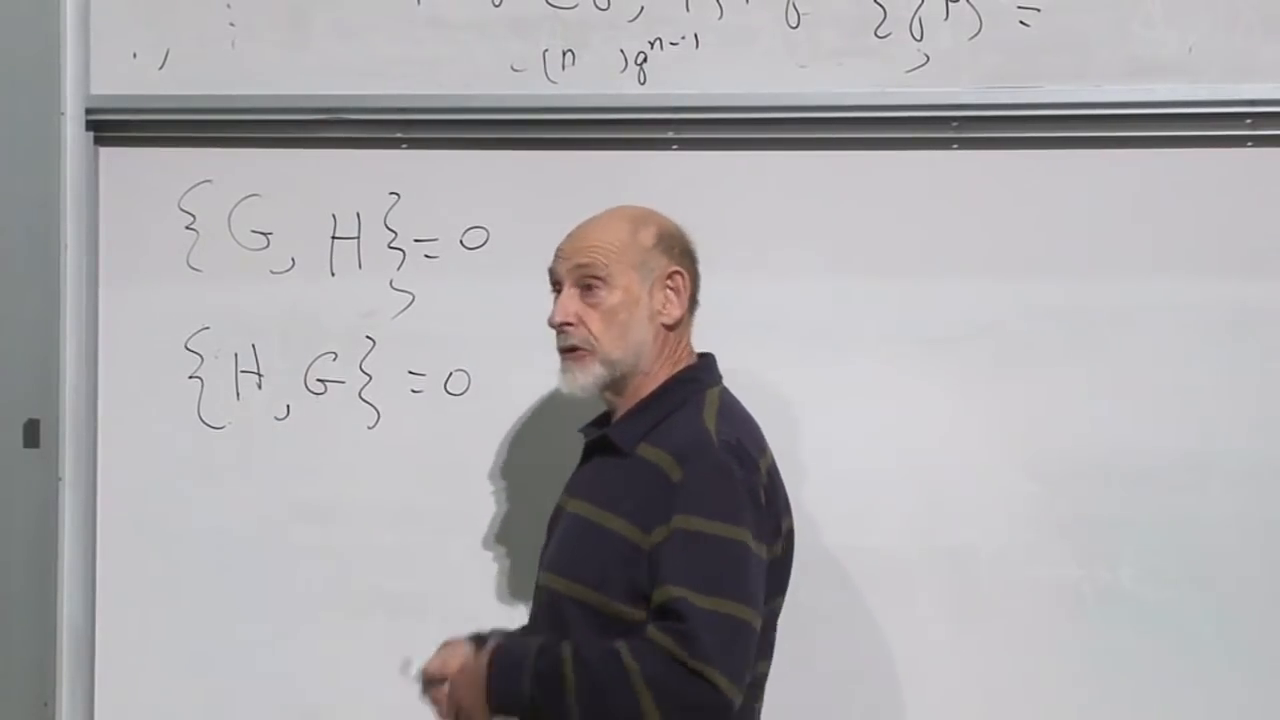
\includegraphics[width=0.82\textwidth]{lecture_08_figure_06.png}
  \caption{同一个消失的括号的两种次序：\(G\)的守恒与\(H\)在\(G\)生成的变换下的不变性。}
  \lectureframe{01:03:05}
\end{figure}

\begin{classroomqa}
  \audiencequestion{如果已知一个守恒量，是否总能恢复出相应的对称性？\lecturetimestamp{01:01:42--01:02:15}}
  \lecturerresponse{在这个哈密顿框架内，可以：将每个相空间变量与\(G\)取括号。所得集合
  \(\delta_GA=\epsilon\{A,G\}\)告诉我们这些变量如何变换。例如，与\(L_z\)的括号揭示出一个旋转，即使事先并不知道这一解释。在更高级的设定中可能出现整体与边界的微妙之处，但此处使用的是局部的无穷小陈述。}
\end{classroomqa}

\begin{classroomqa}
  \audiencequestion{那些括号方程是否告诉我们导致守恒定律的物理运动？
  \lecturetimestamp{00:56:01--00:58:13}}
  \lecturerresponse{不。它们识别的是对称变换，而不是实际轨迹。\(L_z\)的守恒表明旋转对称性；它并不说明粒子沿圆周运动。实际的时间演化由\(H\)生成。与另一个生成元取括号描述相空间中另一个方向的变换。}
\end{classroomqa}

\begin{classroomqa}
  \audiencequestion{是否存在一个不预先假设守恒的一般变换陈述？\lecturetimestamp{01:02:40--01:04:45}}
  \lecturerresponse{有。方程~\eqref{eq:l8-generator-rule}对每个函数\(G\)定义了一个无穷小变换，无论它是否守恒。只有当哈密顿量不变时，它才成为对称性：\(\{H,G\}=0\)。同一条件按相反次序解读，则说明\(G\)是守恒的。}
\end{classroomqa}

\section{角动量代数}

接下来的计算让我们不必在每个转动问题中都拖着粒子坐标。从下式开始
\[
  L_x=yp_z-zp_y,\qquad
  L_z=xp_y-yp_x.
\]
在\(\{L_x,L_z\}\)中，大多数交叉项因指标不构成正则对而消失。幸存的缩并给出
\begin{align}
  \{L_x,L_z\}
  &=\{yp_z-zp_y,xp_y-yp_x\}\\
  &=xp_z-zp_x\\
  &=-L_y.
  \label{eq:l8-lx-lz}
\end{align}
交换次序会去掉负号。轮换坐标得到
\begin{equation}
  \boxed{\begin{aligned}
    \{L_x,L_y\}&=L_z,\\
    \{L_y,L_z\}&=L_x,\\
    \{L_z,L_x\}&=L_y.
  \end{aligned}}
  \label{eq:l8-angular-algebra}
\end{equation}
用指标记号表示，
\begin{equation}
  \{L_i,L_j\}=\varepsilon_{ijk}L_k.
  \label{eq:l8-angular-algebra-index}
\end{equation}

\begin{figure}[htbp]
  \centering
  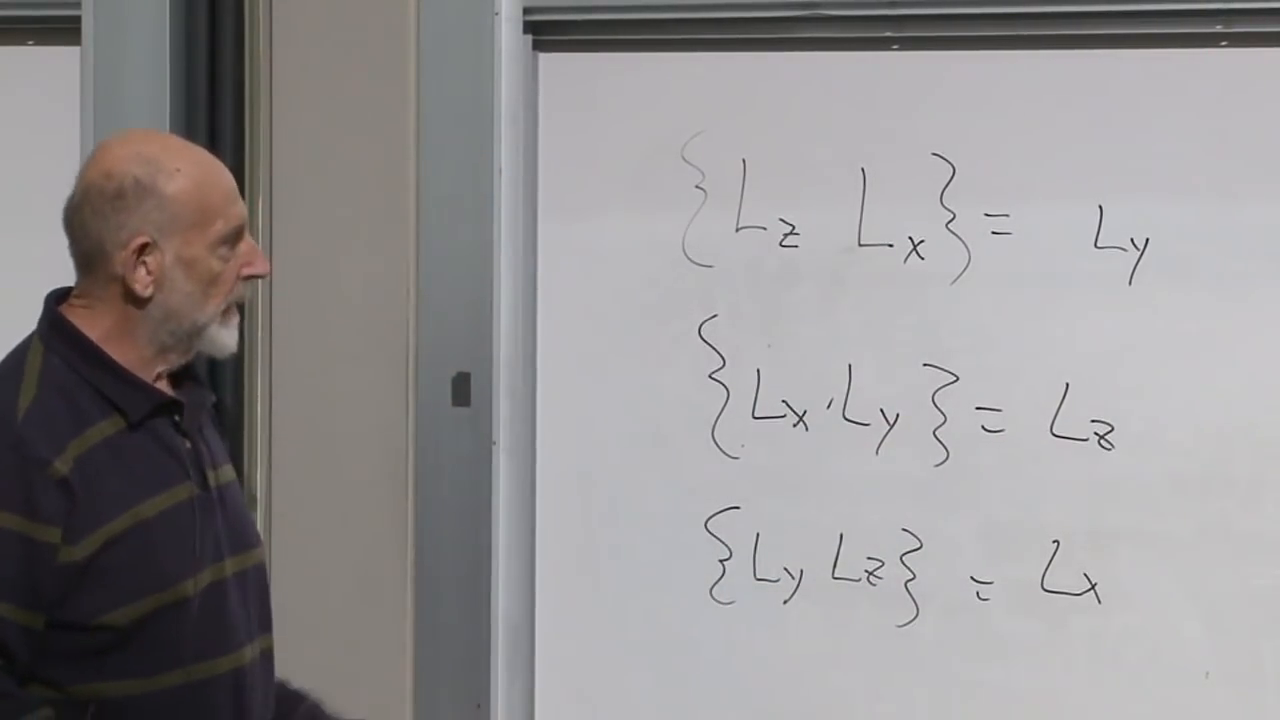
\includegraphics[width=0.82\textwidth]{lecture_08_figure_07.png}
  \caption{三个角动量分量的循环泊松括号代数。}
  \lectureframe{01:10:52}
\end{figure}

这一结果本来也可以预料。既然\(\boldsymbol L\)是矢量，将其\(x\)分量与\(L_z\)取括号，必定给出该分量在\(z\)转动下的无穷小变化，即\(-L_y\)。显式计算证实了这一几何论证。这些方程也是量子角动量对易关系的经典前身。

\section{快速陀螺}

作为一个应用，考虑一个陀螺：一个快速旋转的飞轮，其中心到支点的距离为\(R\)。设\(\boldsymbol r\)从支点指向轮心。飞轮绕其轴旋转得如此之快，以至于其主导角动量始终与该方向对齐。在讲座所用的近似中，
\begin{equation}
  \boldsymbol L=\ell\,\boldsymbol r,
  \qquad
  L_z=\ell z,
  \label{eq:l8-L-parallel-r}
\end{equation}
其中\(\ell=L/R\)被当作常量。与章动或轴的运动相关的较小角动量起初被忽略。

\begin{figure}[htbp]
  \centering
  \begin{tikzpicture}[scale=0.95,>=Latex]
    \coordinate (P) at (0,3.2);
    \coordinate (C) at (3.7,1.55);
    \draw[->] (0,-0.2) -- (0,4.35) node[above] {\(z\)};
    \fill (P) circle (1.7pt) node[left] {pivot};
    \draw[very thick,->] (P) -- (C)
      node[midway,above right] {\(\boldsymbol r\parallel\boldsymbol L\)};
    \fill (C) circle (1.7pt);
    \draw[dashed] (P) -- (0,1.55);
    \draw[dashed] (0,1.55) -- (C);
    \node[left] at (0,1.55) {\(z\)};
    \begin{scope}[shift={(C)},rotate=-24]
      \draw[very thick] (0,0) ellipse (0.65 and 1.35);
      \draw[thick] (0,0) ellipse (0.42 and 0.9);
    \end{scope}
    \draw[->,thick] (2.15,2.85)
      arc[start angle=140,end angle=35,radius=1.65];
  \end{tikzpicture}
  \caption{快速陀螺近似。支点到中心的距离固定，主导自旋角动量始终与轴及\(\boldsymbol r\)对齐。}
\end{figure}

\begin{figure}[htbp]
  \centering
  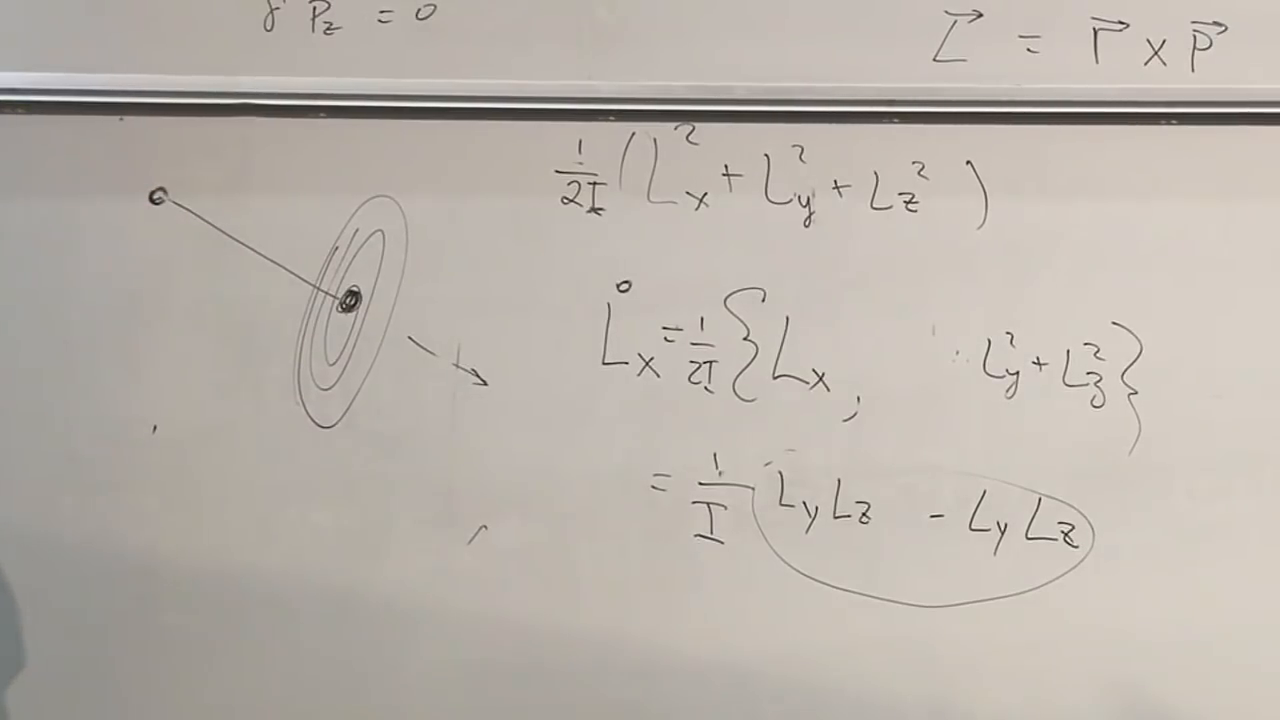
\includegraphics[width=0.82\textwidth]{lecture_08_figure_08.png}
  \caption{黑板上飞轮的草图，连同\(H_{\rm rot}=L^2/(2I)\)以及证明\(\boldsymbol L\)无矩守恒的抵消。}
  \lectureframe{01:18:54}
\end{figure}

\subsection{无重力：为何每个分量都保持不变}

对于简化后的轴对称转子，
\begin{equation}
  H_{\mathrm{rot}}
  =\frac{1}{2I}
  \left(L_x^2+L_y^2+L_z^2\right)
  =\frac{L^2}{2I}.
  \label{eq:l8-rotational-hamiltonian}
\end{equation}
系数是 \(1/(2I)\)，而不是 \(I/2\)；这个笔误是在黑板上写错并改正的。利用式~\eqref{eq:l8-angular-algebra}，
\begin{align}
  \dot L_x
  &=\{L_x,H_{\mathrm{rot}}\}\\
  &=\frac{1}{2I}\left(
    2L_y\{L_x,L_y\}
    +2L_z\{L_x,L_z\}
  \right)\\
  &=\frac{1}{I}\left(L_yL_z-L_zL_y\right)=0.
  \label{eq:l8-free-lx}
\end{align}
循环地，
\begin{equation}
  \dot L_x=\dot L_y=\dot L_z=0.
  \label{eq:l8-free-angular-momentum}
\end{equation}
标量 \(L^2\) 与每个分量 \(L_i\) 的括号均为零；用这套代数的语言来说，它是一个卡西米尔量。因此，不受力矩作用的陀螺仪保持其角动量的大小和方向。

\begin{classroomqa}
  \audiencequestion{这里的转动惯量只是一个数吗？
  \lecturetimestamp{01:14:23--01:15:05}}
  \lecturerresponse{对于这个简化模型，是的。它编码了轮子绕其自转轴的质量分布。一般的刚体有转动惯量张量，以及在主轴下的转动哈密顿量
  \(\sum_i L_i^2/(2I_i)\)。本讲选择更简单的快速对称转子，因为目的是展示泊松括号方法，而不是展开完整的刚体动力学。}
\end{classroomqa}

\subsection{重力与势能的符号}

取竖直坐标 \(z\) 向上为正，并将支点置于原点。轮心的重力势能为
\begin{equation}
  V=Mgz.
  \label{eq:l8-mgz}
\end{equation}
由于 \(L_z=\ell z\)，
\begin{equation}
  V=cL_z,
  \qquad
  c=\frac{Mg}{\ell}=\frac{MgR}{L}.
  \label{eq:l8-potential-lz}
\end{equation}
这里当 \(\boldsymbol L\) 选为平行于 \(\boldsymbol r\) 时 \(c>0\)。如果飞轮朝相反方向自转，\(\boldsymbol L\) 与 \(\boldsymbol r\) 之间的带符号关系反转，相应的带符号进动频率也随之反转。

\begin{figure}[htbp]
  \centering
  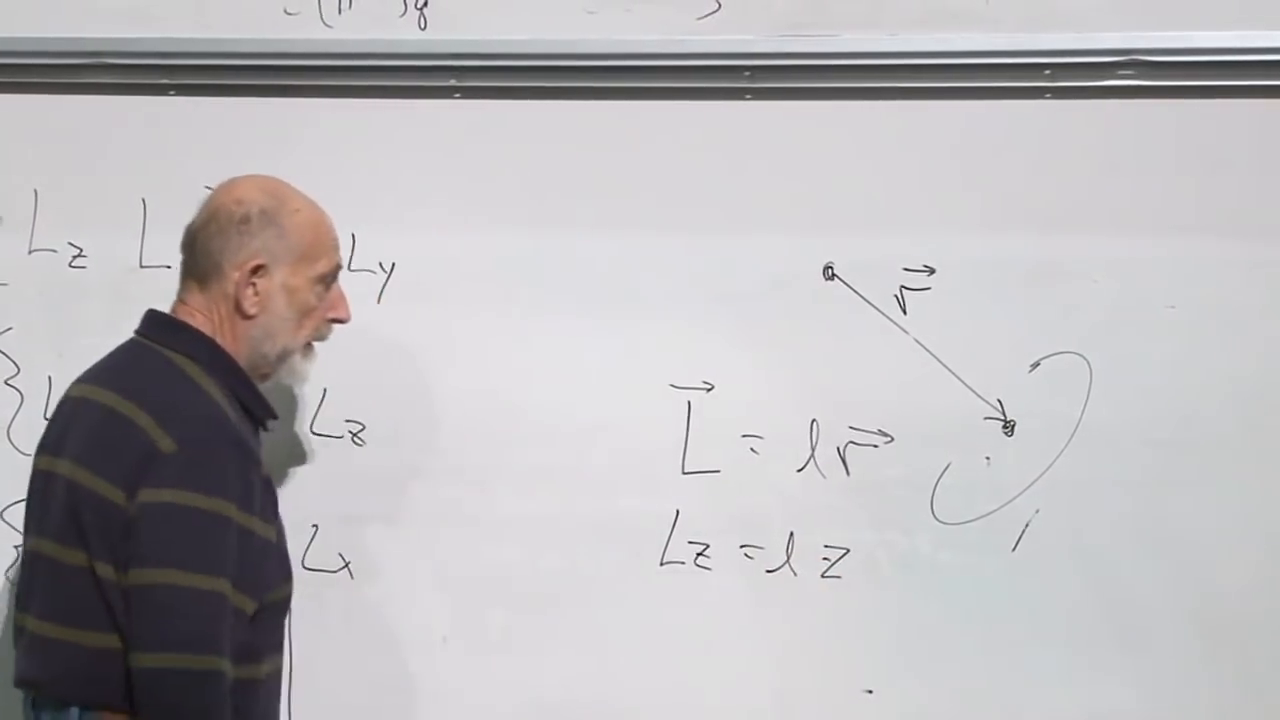
\includegraphics[width=0.82\textwidth]{lecture_08_figure_09.png}
  \caption{\(\boldsymbol L=\ell\boldsymbol r\) 和 \(L_z=\ell z\) 背后的定长几何。}
  \lectureframe{01:25:38}
\end{figure}

\begin{figure}[htbp]
  \centering
  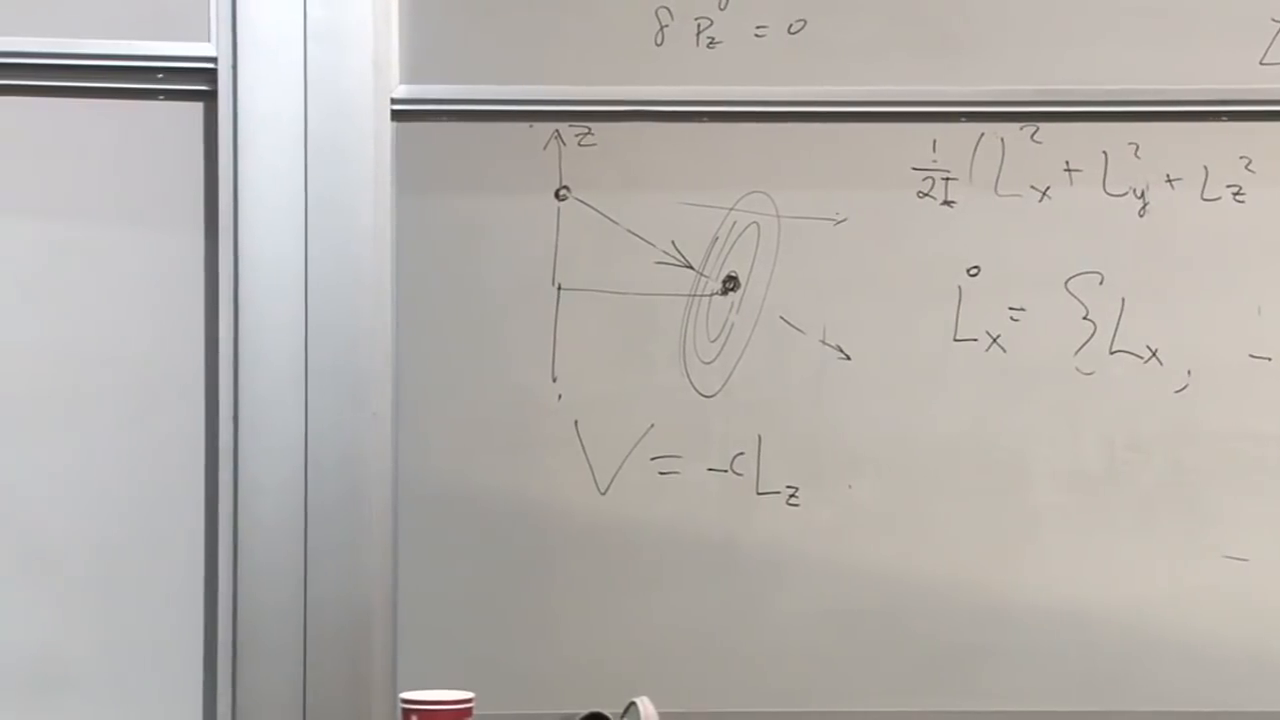
\includegraphics[width=0.82\textwidth]{lecture_08_figure_10.png}
  \caption{黑板上的一个中间状态显示 \(V=-cL_z\)。在将 \(z\) 确定为向上之后，符号会在后面得到修正：当 \(\boldsymbol L=\ell\boldsymbol r\) 且 \(\ell>0\) 时，一致的结果是
  \(V=+cL_z\)。}
  \lectureframe{01:22:43}
\end{figure}

\begin{classroomqa}
  \audiencequestion{为什么高度可以用角动量的一个分量来替换？那条斜线是轴还是位置矢量？
  \lecturetimestamp{01:22:20--01:25:43}}
  \lecturerresponse{那条斜线最好标记为
  \(\boldsymbol r\)，即从固定支点到轮心的矢量。物理轴可能沿它放置，但计算中所用的关系是快速自转近似
  \(\boldsymbol L=\ell\boldsymbol r\)。因此它们的 \(z\) 分量成比例。现场讨论在最终确定这一区分之前，多次更改了标记。}
\end{classroomqa}

\begin{classroomqa}
  \audiencequestion{什么假设使 \(\ell\) 为常量，如果轮心能够径向滑动，又会出什么问题？
  \lecturetimestamp{01:25:43--01:26:38,\allowbreak\ 01:34:22--01:35:00}}
  \lecturerresponse{假设主导的自转远大于与慢运动相关的角动量，并且支点到轮心的距离固定。于是自转大小变化很小，而
  \(\boldsymbol L\) 随 \(\boldsymbol r\) 转动。如果轮心能够径向滑动，\(z\) 就不再以单一常系数与 \(L_z\) 成比例，因此简化哈密顿量 \(V=cL_z\) 将无法描述该运动。}
\end{classroomqa}

\begin{classroomqa}
  \audiencequestion{为什么黑板上先显示负号，后来又显示正号？自转方向有影响吗？
  \lecturetimestamp{01:27:13--01:28:15,\allowbreak\ 01:33:09--01:33:21}}
  \lecturerresponse{最初的符号是现场板书错误，混杂着尚未确定的轴约定。一旦将 \(z\) 定义为向上，
  \(V=Mgz\) 就随高度增加。如果
  \(\boldsymbol L=\ell\boldsymbol r\) 且 \(\ell>0\)，这给出
  \(V=+cL_z\)。反转自转方向会反转带符号的比例关系和进动方向，但不会恢复任意的符号选择。}
\end{classroomqa}

\subsection{由三个短方程得到进动}

完整的简化哈密顿量为
\begin{equation}
  H=
  \frac{1}{2I}\left(L_x^2+L_y^2+L_z^2\right)+cL_z.
  \label{eq:l8-full-gyro-hamiltonian}
\end{equation}
我们已经证明 \(L^2\) 与每个 \(L_i\) 的括号均为零。只有线性项有贡献：
\begin{align}
  \dot L_z&=\{L_z,H\}=0,\\
  \dot L_x&=\{L_x,H\}=c\{L_x,L_z\}=-cL_y,\\
  \dot L_y&=\{L_y,H\}=c\{L_y,L_z\}=cL_x.
  \label{eq:l8-precession-equations}
\end{align}

\begin{figure}[htbp]
  \centering
  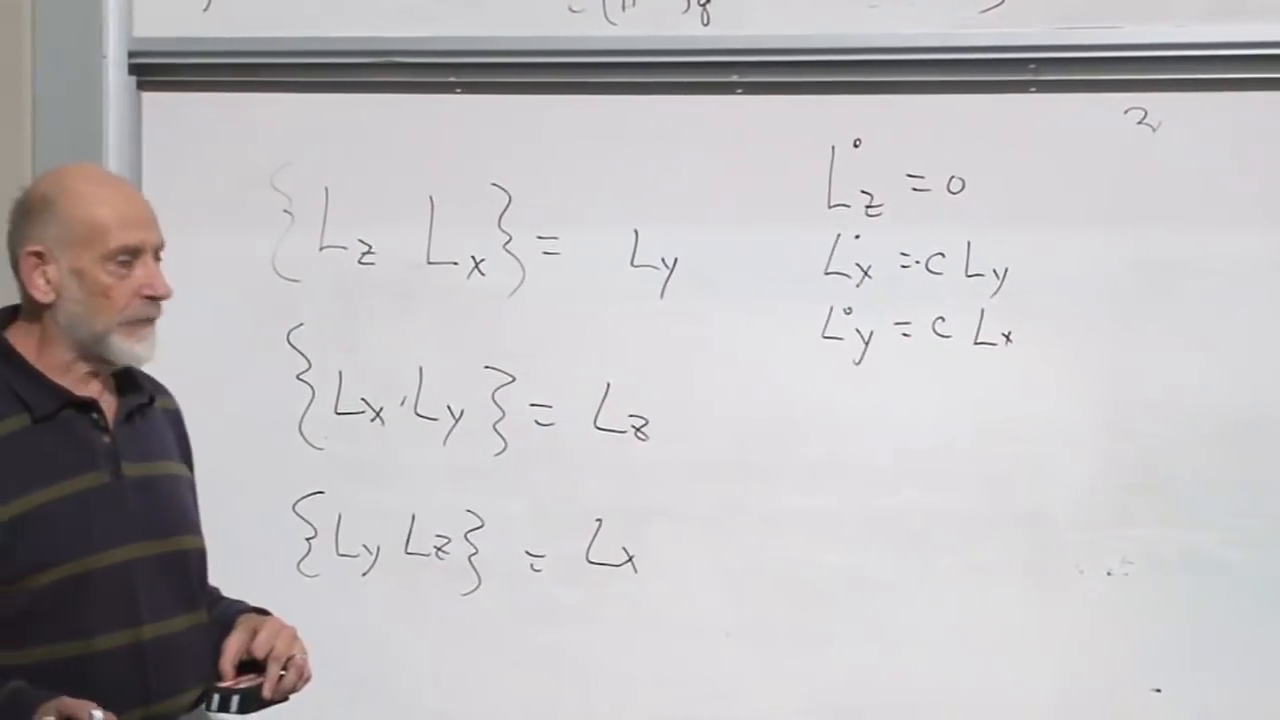
\includegraphics[width=0.82\textwidth]{lecture_08_figure_11.png}
  \caption{最终的分量方程：\(L_z\) 为常量，而
  \(L_x\) 和 \(L_y\) 相互转化。}
  \lectureframe{01:30:35}
\end{figure}

竖直分量和水平方向的大小都是常量：
\begin{equation}
  \frac{d}{dt}(L_x^2+L_y^2)
  =2L_x(-cL_y)+2L_y(cL_x)=0.
\end{equation}
合并水平分量，
\begin{equation}
  L_+=L_x+iL_y,
  \qquad
  \dot L_+=icL_+,
\end{equation}
所以
\begin{equation}
  L_+(t)=L_+(0)e^{ict}.
  \label{eq:l8-precession-solution}
\end{equation}
因此角动量矢量绕竖直轴以角速率 \(|c|=MgR/L\) 进动。在这个理想化的稳态运动中，它的倾角保持不变。

\begin{classroomqa}
  \audiencequestion{在写出进动方程时，转动能量项被忽略了吗？
  \lecturetimestamp{01:35:01--01:35:49}}
  \lecturerresponse{没有。它属于完整哈密顿量，如式~\eqref{eq:l8-full-gyro-hamiltonian} 所示。它对
  \(\dot L_i\) 的贡献恰好为零，因为 \(\{L_i,L^2\}=0\)，这一抵消已在无力矩计算中证明过。学生的问题使这个隐含步骤变得明确。}
\end{classroomqa}

\begin{classroomqa}
  \audiencequestion{匀速进动是一种平衡吗？轻微扰动之后会发生什么？\lecturetimestamp{01:32:38--01:33:08}}
  \lecturerresponse{与其称之为静态平衡，不如称之为稳定运动或定常运动。轻微扰动通常会叠加章动，即倾角的振荡。对于旋转极快的轮子，这种振荡很小，这正是简化处理只保留近似匀速进动的原因。}
\end{classroomqa}

\begin{classroomqa}
  \audiencequestion{进动需要一个支座或一根真实的轴吗？\lecturetimestamp{01:31:49--01:32:38,\allowbreak\ 01:33:49--01:35:00}}
  \lecturerresponse{这个力学模型假定支点到中心的距离固定，因此某种约束提供了支撑。更深入的代数结果则更为普遍：只要角动量有一个哈密顿量项对其某一分量是线性的，同样的括号代数就会产生进动。角动量的微观来源不必是字面意义上装在轴上的轮子。}
\end{classroomqa}

\begin{classroomqa}
  \audiencequestion{这与磁场中电子自旋或核自旋的进动，或者行星轨道的进动是同一回事吗？\lecturetimestamp{01:35:50--01:37:00}}
  \lecturerresponse{磁矩与磁场耦合时，其哈密顿量对自旋分量是线性的，因此遵循同样的角动量代数。核自旋进动是核磁共振的基础。行星轨道近日点的进动是另一种现象，只是恰好共用\emph{进动}这个词；它并不是同一个计算。}
\end{classroomqa}

\begin{classroomqa}
  \audiencequestion{侧装的陀螺仪与旋转的陀螺本质上是同一个物体吗？\lecturetimestamp{01:37:02--01:37:23}}
  \lecturerresponse{是的。区别主要在于几何用语：当自转轴从支座向侧方伸出时，通常称之为陀螺仪；当它接近竖直时，则称之为陀螺。角动量和力矩的结构是相同的。}
\end{classroomqa}

\section{计算所完成的事}

没有引入欧拉角，也没有追踪轮子每一部分对应的坐标。一旦\[
  \{L_i,L_j\}=\varepsilon_{ijk}L_k
\]已知，所关心变量的方程便直接随之得到。这正是所要展示的威力。谐振子表明，泊松括号能够重现熟悉的动力学。角动量则表明，它们所能做的远不止于此：
\begin{itemize}
  \item 一个守恒量生成与之相伴的无穷小对称性；
  \item \(G\)的守恒与\(H\)的不变性是
  \(\{G,H\}=0\)的两种读法；
  \item 可观测量的代数可以自封闭，从而无需回到微观坐标即可求解动力学；
  \item 一个对某一角动量分量线性的哈密顿量会产生绕该轴的进动。
\end{itemize}
本讲在给出一般刚体的完整欧拉方程之前便告结束。其较窄的结论却已经完备：恰当的生成元及其泊松代数以惊人的经济性同时揭示了对称性与运动。